%
% File acl2012.tex
%
% Contact: Maggie Li (cswjli@comp.polyu.edu.hk), Michael White (mwhite@ling.osu.edu)
%%
%% Based on the style files for ACL2008 by Joakim Nivre and Noah Smith
%% and that of ACL2010 by Jing-Shin Chang and Philipp Koehn


\documentclass[11pt]{article}
\usepackage{acl2012}
\usepackage{times}
\usepackage{latexsym}
\usepackage{amsmath}
\usepackage{multirow}
\usepackage{url}
\usepackage{subfig}
\usepackage{graphicx}
\DeclareMathOperator*{\argmax}{arg\,max}
\setlength\titlebox{6.5cm}    % Expanding the titlebox

\title{Finding Structure in Gradable Adjectives From Vector-Space Models and Human Judgment}

\author{
  Kevin Leung \\
  Stanford University \\
  {\tt kkleung@cs.stanford.edu}}

\date{}

\begin{document}
\maketitle
\begin{abstract}
Gradable adjectives can be classified according to their scale structures, which have been theorized to determine whether the adjectives accept certain degree modifiers. By presenting experimental evidence, we examine where this theory explains acceptability judgments and where it needs to be extended . Further, we attempt to extend this theory into general usage by examining counts from a large corpus. We show that although the theory predicts most acceptability judgments, it is also confounded by other senses of these same degree modifiers and gradable adjectives, such as speaker confidence and quantification, as well as specific characteristics of words and the register of the data.
\end{abstract}

\section{Introduction}

Gradable adjectives (GAs) are adjectives that accept degree modifiers (DMs), which determine to what extent the adjective describes the object. For example, \textit{large} is gradable because someone can be \textit{very large} or \textit{extremely large}. On the otherhand, \textit{metallic} is not gradable because an item cannot be \textit{very metallic} or \textit{slightly metallic}. Kennedy and McNally \shortcite{kennedymcnally} argue that GAs can be further separated into types depending on their scale structure. These classes also determine the set of DMs that the GAs accept.

We evaluate this theory and determine where it sufficiently explains acceptability judgments and where it needs to be extended to fit judgment. To do this, we use 3 types of data. First, we apply the theory directly to specific DM-GA pairs upon whether they are acceptable or not. Second, we gather human judgments of the naturalness of the same pairs and find patterns within those. Finally, we count instances of adverbial modification in The New York Times Newswire Service corpus from English Gigaword to generate vector-space models (VSMs) of the words. By comparing all three datasets, we explore how the theory applies in actual judgments and usage.

In this paper, we will first cover the theory of GAs and scale structure and other related works. Next, we will describe the experiments and results specific to the experiments. Third, we will describe the vector-space models tested and results specific to those models. Then, we will compare and discuss the results from all 3 sources of data. Finally, we will propose some further exploration and research to be done based on our findings.

\section{Kennedy and McNally 2005}

First, we'll begin with background on the theory being evaluated. Kennedy and McNally \shortcite{kennedymcnally} present a linguistic theory on the types of adverbs that can modify GAs. Unlike nongradable adjectives, GAs can describe its object at differing degrees, depending on the modification. This theory argues that GAs accept degree modification according to the scale structure that they fit.  A scale is a total ordering over degrees for the concept being expressed by an adjective. These scales come in various types depending on whether they have minimum and maximum values. Thus, a scale can be open (no minimum or maximum), closed (minimum and maximum), lower closed (only minimum), and upper closed (only maximum). These correspond to different possible DMs that they accept. For example, proportional modifiers work with adjectives with closed scales.

\begin{enumerate}
\item Chris thought the football stadium was \textit{half full}.
\item ?? Bill bought a \textit{half expensive} shirt.
\end{enumerate}

Another example of a scale-constrained modifier is \textit{slightly}, which relates to a minimum value.

\begin{enumerate}
\item Chris rode his bike on the \textit{slightly wet} road.
\item ?? Bill made many \textit{slightly accurate} comments during class.
\end{enumerate}

These scale structures can also be thought to vary on the standard of comparison. Some adjectives, such as \textit{expensive} depend on the context, while others, such as \textit{full} do not. They argue that context-dependent (relative) adjectives correlate to completely open scales, whereas context-independent (absolute) adjectives correlate to closed scales. 

Moreover, they claim that scale structures are not only a helpful way for us to conceptualize language, but are actually the cognitive basis for how we think about language. Thus, scale structures are important in human reasoning, and this theory has consequences on how language shapes thought.

To evaluate this theory, we extracted 49 GAs and 14 DMs that are stated as belonging to specific types \cite{kennedymcnally} \cite{kennedy07}. We then labeled the pairs according to Table \ref{tab:theory-table}.

\begin{center}
\begin{table*}[ht]
\hfill{}
\begin{tabular}{|l|l|l|l|l|}
\hline & \bf Proportional & \bf Maximizing & \bf Minimizing & \bf Intensifier \\ \hline
Closed scale & Yes & Yes & Somewhat & Somewhat \\ \hline
Upper closed scale & Somewhat & Yes & No & Somewhat \\ \hline
Lower closed scale & No & No & Yes & Somewhat \\ \hline
Open scale & No & No & No & Yes \\ \hline
\end{tabular}
\hfill{}
\caption{\label{tab:theory-table} Acceptability judgments for types of DMs and the scales that correspond to types of GAs. Although the theory doesn't disallow the pairs labeled with "Somewhat", it does indicate that they should occur less frequently than other, more acceptable pairs.}
\end{table*}
\end{center}

\section{Related Work}

Rooth et al. \shortcite{rooth} implemented a EM-based clustering algorithm on co-occurrence frequencies in large corpora to discover semantic classes. Boleda Torrent and Alonso i Alemany \shortcite{boleda} used clustering to find adjective classes in Catalan based on several simple features, including the POS within a five-word window and a few handwritten rules. Hatzivassiloglou \shortcite{hat} tested several methods of extracting noun-adjective relationships from a corpus and clustered those result to find semantic classes for adjectives. Maas et al. \shortcite{maas} improves the accuracy of vector-based word representations with sentiment labels. Their approach combines corpus data and expert labels to learn. Many experiments have been performed to find acceptability judgment data, particularly in syntax, that are modeled after methods from experimental psychology \cite{sprouse}.

Syrett and Lidz \shortcite{syrett} performed a small corpus analysis to find a difference in degree modification of open and closed scale gradable adjectives to show that there are usage differences for children to observe and learn from. Their method is similar to our approach with vector-space models, and we aim to improve upon it. First, we make further distinctions between the types of closed scales and how modification should occur with each one separately. Second, we use a larger (yet still manageable) dataset to move away from prototypical examples and see how well this theory applies to GAs in general.

\section{Human Judgment}

\subsection{Experiment 1}

In our experiments, we wanted to directly evaluate the theory, and we had several specific goals with this experiment. First, we wanted to determine if people made a distinction between the "naturalness" and "grammaticality" of certain pairs. Although the theory makes no distinction between these two concepts, it is possible that certain phrases are entirely meaningful and grammatically correct but simply unnatural or uncommon for pragmatic or otherwise theoretically unmotivated reasons. Second, we wanted to see how this theory worked broadly to expand upon the Syrett and Lidz \shortcite{syrett} work.

\subsubsection{Methods}
The stimuli was 100 random pairs of DMs and adjectives (mostly gradable, but also some nongradable) from a list of 134 adjectives and 40 adverbs selected from a list of the most common adverbs and adjectives in the English language. All of adjectives and adverbs were labeled by the author according to the types in Table \ref{tab:theory-table} and reviewed by an expert in gradable adjectives.

The subjects were 47 native English speakers (19 male, 28 female, from ages 19 to over 60). 3 additional subjects were excluded from results due to inattentiveness. All subjects were recruited via Mechanical Turk, where the study was conducted, and they were paid for approximately 10 minutes worth of work. The subjects were allowed to proceed at their own pace, and their environment was otherwise not controlled.

Upon accepting the experiment, each subject was randomly assigned to either the "grammaticality" or the "naturalness" condition and received instructions on the task. After that, all 100 stimuli were presented, 1 at a time in a randomized order for each subject. On each trial, the subject was presented with the adverb-adjective pair and prompted to rate on a scale of 1 to 9 the acceptability of the pair. Based on previous methods in experimental syntax \cite{sprouse}, the subject either saw either "Does this expression sound meaningful to you?" in the "grammaticality" condition or "How natural does this expression sounds to you?" in the "naturalness" condition. Upon selection and clicking next, the next trial began. After completing all 100 trials, the subject filled out a short survey.

\subsubsection{Results and Discussion}

We first calculated z-scores within each subject to normalize for different usages of the scale. These scores were then averaged together to determine an aggregated acceptability rating for each stimulus. The results of the grammaticality and naturalness conditions had a cosine similarity of .9666. This suggests that subjects didn't distinguish between the intent of the 2 conditions, which gives more validity to the model analysis in the next section based on usage. The results from the 2 conditions were collapsed in further analysis because they weren't significantly different.

The results were compared to the theory predictions by thresholding the z-scores at 0, where a pair was accepted if the z-score was above 0, and rejected otherwise. Using this scheme, the results and theory agreed on 56/86 (65\%) of trials that involved both a DM and a GA. By a two-tailed binomial test, we reject the null hypothesis (p=.0067) that acceptability was determined randomly. Given that these judgments should be determined by the theory, this agreement is still lower than expected.

Although the results suggest that the theory predicts some aspects of the data, we were unable to further explore this question for 2 reasons. First, the stimuli set wasn't coherent enough for structured comparison because we only gathered data for 100 of 5360 possible pairs. Second, there was some disagreement and low confidence in the labels for the adjectives and adverbs. Even though the labels were based on the theory presented, an easy criticism of our data is that the theory was misapplied to these words.

\subsection{Experiment 2}

The agreement with the theory predictions in Experiment 1 was lower than we expected, and we hypothesized that there were smaller subsets of the data that had significantly higher and lower agreement. We determined that we needed to gather judgments on a narrower set of data to determine for what cases the theory accurately predicted acceptability and where it didn't fully explain the results.

\subsubsection{Methods}
The stimuli selected was all pairs of the 49 GAs and 14 DMs (686 total pairs) that Kennedy and McNally explicitly labeled in their paper. This data fill out a complete matrix for all pairs with expert labels. These 686 words were randomly divided into 49 sets of 98 stimuli each, where each stimuli appeared in exactly 7 distinct sets. This division ensures that all stimuli received an approximately equal number of evaluations while avoiding any bias from any particular set of words (e.g. simply dividing the 686 stimuli into 7 sets of 98 stimuli).

The subjects were 310 native English speakers. 30 additional subjects were excluded from results due to inattentiveness. All subjects were recruited via Mechanical Turk, where the study was conducted, and they were paid for approximately 10 minutes worth of work.

Each subject received 1 of the 49 stimuli sets generated in random order. The instructions and trials were presented using the text from the "naturalness" condition of Experiment 1. Otherwise, the procedure was identical to Experiment 1.

\subsubsection{Results and Discussion}

Most of the results will be discussed below in combination with the theoretical prediction and the VSM. One notable adjustment necessary was the removal of the DMs \textit{well} and $much$ from further analysis. The rest of the DMs resulted in nuanced ratings, with both high and low ratings across the GAs, \textit{well} and $much$ received negative z-scores with in every pair, with most being below -1. For comparison, only 17 of the other 588 pairs had a z-score below -1.

A further consequence of their inclusion in the dataset is that they may have caused an anchoring effect in the subjects over the course of their trials. Although z-scores normalize for different uses of the scale, we lost sensitivity as \textit{well} and \textit{necessary} may seems extremely unacceptable compared to other less unacceptable pairs that will receive relatively higher scores because of the anchoring. Even so, we used the scores calculated with \textit{well} and \textit{much} included and believe that the analysis remains valid despite removing them later. Unfortunately, this means that \textit{half} is the only proportional modifier left, and \textit{partially} and \textit{slightly} are the only 2 DMs with a minimum standard. Thus, data aggregated from those types should be treated with more caution. 

One possible problem with the design of this study is that by presenting the pair out of context, we were unable to constrain how subjects considered the pair. For example, Kennedy and McNally \shortcite{kennedymcnally} point out that relative adjectives are acceptable when the standard of comparison is fixed. Someone cannot be "half tall," but he or she can be "half as tall as Yao Ming." WIthout fixing the context, we leave open the possibility that subjects may be embedding the pair in qualifying phrases or simply imagining situations to use it.

In the following sections, we will be using the results from Experiment 2 for comparison.

\section{Vector-Space Model}

As well as using acceptability judgment, we also wanted to see if we could find the same effect by mining a large corpus for other DM and GA pairs. Although human judgment is the ground truth for the theory in question, corpus work was motivated by several reasons. First, human judgment is relatively expensive to get: it requires that the entire dataset be hand-labeled by multiple subjects to ensure significance. Corpus data is only as expensive as counting occurrences. Second, further research on a different set of words requires that human labeling happen again. With a large enough corpus, all combinations desired should be represented, and the frequency of certain pairs should be meaningful. Third, experimental conditions may not entirely reflect true acceptability of certain pairs. As discussed above, there are other factors, such as anchoring effects, that may influence acceptability judgments. Corpus data reflects true usage and should properly capture judgments in a naturalistic setting.

We caution readers that Kennedy and McNally \shortcite{kennedymcnally} don't make predictions about corpus usage, and thus, this data cannot be used to evaluate their theory directly. Corpus statistics, however, should reflect acceptability, albeit noisily. 

\subsection{Methods}
We used The New York Times Newswire Service corpus from English Gigaword, which includes approximately 915 millions words over approximately 1.3 million documents gathered from 1994 to 2002. From that, we extracted about 40 millions instances of adverbial modification using the Stanford Dependency Parser \cite{marneffe}. In previous work, we used bigram counts from the Web1T corpus to also find examples of adverbial modification. Between these 2 sets, there was a similarity of .84. Although the similarity is high enough that we believe the results will generalize, there may be some results specific to this corpus.

From this set of dependencies, we further narrowed the data down to the set that is relevant for this study. The first set contained exactly the 49 GAs and 14 DMs used in Experiment 2, which allows for direct comparison between all 3 sources of data. The second set contained all adjectives and adverbs from Experiment 1 and 2 combined so that the larger dataset may generate a different, more general representation of the words.

With all of counts, we assemble a word-by-word matrix, with each row representing an adjective and each column representing an adverb. These rows and columns are the vector representations for the words: similar adjectives should have similar vectors because they are modified by adverbs in the same way. By limiting the adverbs to only DMs in our application, the resulting representations for the adjectives should align with different classes because the classes all have unique signatures for acceptable modification.

Although the raw frequency counts from the corpus should encode these properties, additional weighting is needed to deal with 2 main problems. First, the difference in frequency is exaggerated in a way similar to Zipf's Law. Although \textit{very} is very common, it is unlikely to be several times more acceptable with adjectives than other adverbs. These differences in frequency should be reduced. Second, there are still issues of data sparsity even with large corpora. In the set of words from Experiment 2, 141 of 686 (20\%) of the pairs had 0 occurrences, and an even higher percentage of 0s likely occur with larger data sets of less frequent words. To deal with both of these problems, we applied several different weighting schemes and compared them to human ratings to find the best correlation.

%We also tried to cluster the adjectives using several different clustering algorithms: $k$-means, hierarchical clustering, mixture of gaussians, and spectral coclustering \cite{coclustering}, with principal components analysis (PCA) applied where necessary. By comparing the representations, different clustering algorithms find sets of vectors that are similar and group them together. If these vectors do encode the classification desired, they should form clusters that align to particular classes.

\subsection{Results and Discussion}

%\begin{table}[h]
%\begin{center}
%\begin{tabular}{|l|l|l|l|}
%\hline \bf Cluster 1& \bf Cluster 2 & \bf Cluster 3 & \bf Cluster 4 \\ \hline
%completely & extremely & absolutely & rather \\ 
%half & perfectly & & \\ 
%much & pretty & &  \\ 
%partially & quite & &  \\ 
%slightly & very & & \\ 
%totally & & & \\ 
%well & & & \\ \hline
%\end{tabular}
%\end{center}
%\caption{\label{tab:adv-clusters} Adverb clusters found by coclustering. }
%\end{table}
%
%Overall, the clustering algorithms where unable to extract any meaningful clusters and largely separated only one or two apparently exceptional adjectives from the rest of them. One notable result was the clustering over the adverbs from coclustering in \ref{tab:adv-clusters}. Cluster 1 contains only DMs for closed scales, whereas Cluster 2 contains intensifiers, except for \textit{perfectly}. \textit{Absolutely} and \textit{rather} may be exceptional in other ways.
%
%Previous work had difficulty finding meaningful clusters out of the resulting vectors, and this approach continues to be difficult, even with a presumably more compact dataset. Many times, the resulting clusters would be 1 or 2 words in most clusters, then the rest of them in 1 large cluster. This suggests that in this space, individual differences of usage for particular words are much more salient than the classes of GAs that we're hoping to extract. Further attempts to factor out these quirks (beyond simply removing the exceptional words) would likely cause more and more information loss in this data. As such, it seems that more detailed analysis of the data will be more fruitful in the short-term.



\begin{figure*}[ht]
\begin{center}
  \subfloat[Correlation of different weightings with Experiment 2 results]{\label{fig:weightings}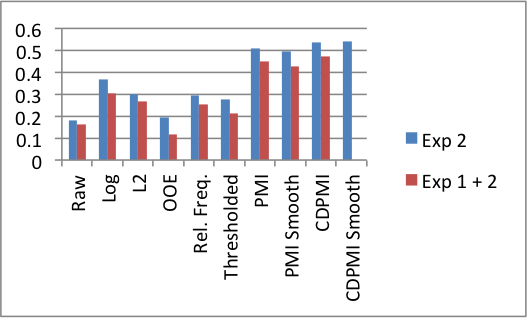
\includegraphics[]{weightings.png}}
~
  \subfloat[Average rating for GAs with scales closed above]{\label{fig:closed-above}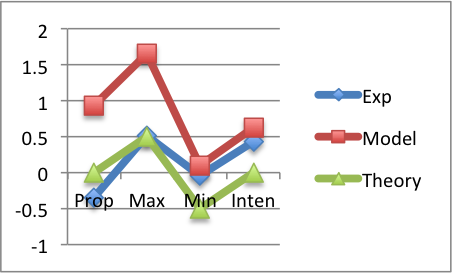
\includegraphics[]{closed_above.png}}
  
  \subfloat[Average rating for GAs with scales closed below]{\label{fig:closed-below}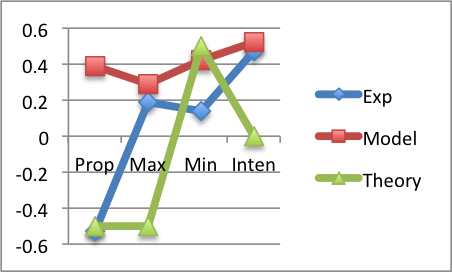
\includegraphics[]{closed_below.png}}
~
  \subfloat[Experiment ratings for \textit{closed} (red) and \textit{asleep} (blue) with DMs across the x-axis.]{\label{fig:closed-asleep}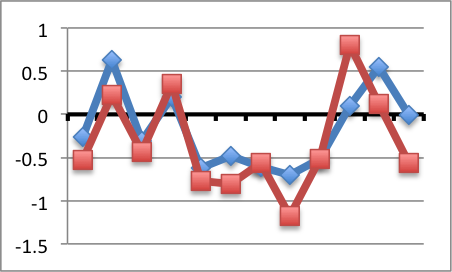
\includegraphics[]{closed_asleep.png}}  

  \caption{Various results charts.}
  \label{fig:all}
\end{center}
\end{figure*}

Figure \ref{fig:weightings} shows the pair-by-pair correlation calculated between different weighting methods and the results from Experiment 2. Between the larger (Experiment 1 + Experiment 2) and smaller (Experiment 2 only) datasets, the smaller set generated better correlations with experiment results. Although the larger set gives more data for the weighting schemes to normalize by, it's possible that much of this data was uninformative for the task at hand. The final vector representations may be more accurate holistically, but on the naturalness task for GAs, the smaller set avoids some of the potentially confounding characteristics introduced by less coherent data.

The variants of pointwise mutual information (PMI) perform the best, with the addition of both contextual discounting and Laplace smoothing performing the best ($r = .5397$), with taking the $\log$ of the counts performing next best after the PMI variants. This is consistent with the exponential increase in usage with respect to actual acceptability. Among the variants, the results were close, but the combination of contextual rescaling and smoothing appeared to do the best. Contextual rescaling increases the weight towards values with more evidence and away from infrequent data that may be heavily skewed. Smoothing deals with the problem of data sparsity as 0s in the data are difficult to assign. Conventionally, they are replaced with a PMI of 0, but in our interpretation, this roughly means "neither acceptable nor unacceptable". This problem significantly hurts the correlation with experiment data. To compensate for this in later analysis, a PMI rating of 0 is treat as a "not accept".

This particular combination is somewhat contradictory, as smoothing increases the weight on infrequent events, which contextual rescaling will then discount. One possible reason for the success of this combination is that human judgments tended to have more intermediate values (especially z-scoring and averaging across subjects), and the smoothing was necessary to some degree to push weight towards infrequent events, while contextual rescaling mainly addressed other aspects of the data. Even though the improvment was relatively small, we will use PMI with contextual discounting and smoothing in further analysis.

One caveat to note with this approach is that although this weighting scheme works, it theoretically doesn't capture the qualities that we want. PMI is intended to find variation from the norm for the 2 variables (in this case, adjective and adverb frequency) in specific combinations. As such, it enforces balance where it isn't desired. For example, \textit{very} is very frequent with all adjectives and should have universally high acceptability ratings. Unfortunately, PMI necessarily needs to decrease the weight on some of the adjectives that \textit{very} associates with since the values are calculated relative to other uses of \textit{very}, not in relation to the dataset holistically. Contextual discounting addresses this by reweighting towards the high counts, but even that was intended to reduce weight on more reliable counts, not boost high counts for their own sake. The difference is subtle, and although PMI does perform the best out of the weighting schemes used, this application may require a new method of weighting.

\section{Results}

To find agreement between the theoretical predictions, experiment data, and model data, we needed to discretize the continuous ratings into the labels from Table \ref{tab:theory-table}. To divide the data into the 3 classes, we maximized agreement by varying a threshold value $\alpha$ such that all ratings above $\alpha$ would accept, all ratings below $-\alpha$ would reject, and all ratings in-between would be "somewhat acceptable." Unfortunately, this scheme led to $\alpha=0$, so almost nothing would be classified as "somewhat acceptable." From then on, we treated "somewhat acceptable" as "acceptable" and found $\alpha$ as a simple threshold between accept and reject. As expected for z-scores and PMI values, we maximized agreement with $\alpha$ at or very near 0 in all cases. These are shown in Table \ref{tab:agreement}, with further segmentation of these numbers in Table \ref{tab:rating-agreement} and \ref{tab:model-agreement}.

\begin{table}[h]
\begin{center}
\begin{tabular}{|l|l|l|l|}
\hline & \bf Theory & \bf Human \\ \hline
Human & 512 (.75) & N/A \\ \hline
PMI & 485 (.71) & 505 (.74) \\ \hline
PMI Smooth & 472 (.69) & 491 (.72) \\ \hline
CDPMI & 485 (.71) & 505 (.74) \\ \hline
CDPMI Smooth & 491 (.72) & 513 (.75) \\ \hline
\end{tabular}
\end{center}
\caption{\label{tab:agreement} Agreement between data over 686 pairs. }
\end{table}
\begin{table}[h]
\begin{center}
\begin{tabular}{| l | l | l | l | l | l | }
\hline
& max & inten & prop & min & total \\ \hline
closed & .78 & .8 & .44 & .72 & .75 \\ \hline
max & .93 & .76 & .9 & .45 & .78 \\ \hline
min & .3 & .88 & .8 & .7 & .65 \\ \hline
open & .64 & 1 & 1 & .68 & .83 \\ \hline
total & .65 & .89 & .84 & .64 & .77 \\ \hline
\end{tabular}
\end{center}
\caption{\label{tab:rating-agreement} Agreement proportions from Experiment 2 and theory. }
\end{table}
\begin{table}[h]
\begin{center}
\begin{tabular}{| l | l | l | l | l | l | }
\hline
& max & inten & prop & min & total \\ \hline 
closed & .61 & .44 & .44 & .5 & .51 \\ \hline
max & .85 & .74 & .5 & .65 & .74 \\ \hline
min & .63 & .76 & .8 & .3 & .64 \\ \hline
open & .93 & .84 & .55 & .85 & .85 \\ \hline
total & .79 & .73 & .57 & .63 & .72 \\ \hline
\end{tabular}
\end{center}
\caption{\label{tab:model-agreement} Agreement proportions from the model and theory. }
\end{table}

We can also see the variation across categories by averaging all ratings within each GA and DM type for both the experiment and model data, which can be compared to the predicted acceptability from the theory. 2 of these are seen in Figure \ref{fig:closed-above} and \ref{fig:closed-below}. Note that all 3 of these data sources are on different scales, so the trend is more important than the exact values. In Figure \ref{fig:closed-above}, we can see that all 3 data sources agree on the general of the acceptability of GAs with scales that are closed above. This, however, doesn't hold in Figure \ref{fig:closed-below}, where the theory predicts that maximum standard DMs are unacceptable with GAs closed below, yet both the experiment and model data appear to accept them.

\section{Discussion}

In the results, we discussed some general trends and summary statistics that indicate that the theory does explain much of the judgments. Table \ref{tab:agreement} shows that the theory, experiment, and model agree on more than 70\% of the pairs. In Table \ref{tab:rating-agreement} and \ref{tab:model-agreement}, however, there are a few discrepancies that should be explained, as well as some observations from data that did not fit here \footnote{All files, including further data, are available at https://github.com/StoicLoofah/gradable-adjective-corpus-analysis, for further analysis}.

Agreement with the theory on proportional modifiers was generally low, though \textit{half} was the only proportional modifier (\textit{well} was removed). Specifically, \text{half} had positive experiment ratings for only \textit{open, closed, full, empty, asleep, awake,} and \textit{bent}. The first 3 are all opposite pairs, though \textit{bent}'s opposite, \textit{straight}, is not present. 

It's possible that in judging \textit{bent}, subjects had an implicit sense of a maximum bend (such as a person touching their toes) that made this acceptable. This may be a pseudo-maximum on the scale, where people assume a default maximum but also allow for this to become open-ended when prompted. For example, a wire may be \textit{half bent} when it in a 90-degree bend, but when it is "maximally" bent at 180 degrees, someone would happily bend it more if prompted. A similar example from the data is \textit{flexible}, a relative adjective that was accepted with all DMs except for \textit{half}. Although the meaning of \textit{absolutely flexible} isn't well-defined by the scale structures alone, it's possible that people have default standards for flexibility (such as an Olympian gymnast) that are useful without explicit mention but can be modified beyond the default standards.

\textit{Asleep} and \textit{awake} are also unusual in that they are labeled as being upper closed and lower closed, respectively, so neither should be acceptable with a proportional modifier. Exactly how \textit{half} modifies these words isn't clear intuitively, either, as the scale isn't well-defined.

Given these facts, the 44\% agreement between the experiment and theory on proportional modifiers with closed scales, and the generally poor agreement of proportional modifiers from the model, it at least appears that \textit{half} is not a good determiner for whether a GA is closed. Unfortunately, we cannot make further generalizations about proportional modifiers. 

Another interesting result was that \textit{closed} and \textit{asleep} had very similar vectors in the experiment ratings that were very different from any other vectors (Figure \ref{fig:closed-asleep}). Most notably, neither of them were accepted by any of the 5 intensifiers, whereas over 95\% of all GA-intensifier pairs were accepted. This suggests that \textit{closed} and \textit{asleep} are not generally gradable like the rest of the GAs in this set, though it is not clear how. Regardless, it appears that \textit{closed} and \textit{asleep} should belong to the same type, and it might be that \textit{asleep} has a closed scale.

In the results, we mentioned the large discrepancy between theory predictions and actual data for maximum standard DMs and lower closed adjectives. There are several findings about maximum standard DMs that may explain this result.

A major difference between the experiment and model ratings was on \textit{totally}, which was acceptable with all absolute and most relative GAs in the experiment, but not acceptable with almost all lower closed and relative GAs in the model. Many of these negative ratings from the model came from 0 or extremely low counts in the data. This difference may come from the different registers between naturalness and newswire data. The corpus counts come from The New York Times, which has a style guide and standards for English usage that likely disallow \textit{totally} in many circumstances. \textit{Totally} in common usage, however, can be a slang hyperbole, such as a new pop song being "totally rad." In this case, the corpus data, although presumably derived from human judgment, is actually closer to the intended meaning than the experiment data.

Some of the pairs that were accepted by humans but not predicted may be the result of different sense for the modifiers and adjectives in question. For example, \textit{completely} was accepted for all lower closed GAs except "bumpy" (which had a rating of -.01) and almost half of the relative adjectives. Its use with some of the adjectives, however, may not be in a graded sense. For example \textit{completely dirty} likely doesn't mean "maximally dirty", but perhaps "dirty in every way", so a table with every inch covered in dust would be \textit{completely dirty}. This use of \textit{completely} is closer to quantification. For another example, \textit{pleased}, a relative adjective, was accepted by all maximum-standard DMs. If someone tells me that they are "absolutely pleased with my results", they more likely mean that they are "absolutely sure that they are pleased" and not "pleased to the absolute degree." The theory for GAs does not cover, and is not intended to cover, cases of speaker confidence, and judgments of these 2 uses need to be disambiguated.

It has been argued that \textit{possible} and \textit{likely} both function upon the same scale structure, except that \textit{possible} has a minimum value and \textit{likely} does not, so the difference between these should be apparent with ratings on minimum standard DMs, \textit{partially} and \textit{slightly}. Although \textit{possible} is less unacceptable with the minimum standard DMs (-.46 and -.21) than \textit{likely} (-.95 and -.40), these are still both unacceptable to humans (and the model as well), which gives little evidence for a difference.

\section{Conclusion}

Overall, it appears that the Kennedy and McNally theory captures much of the data on acceptability judgments, both from human judgments on naturalness and actual usage from corpus data. Even so, DMs and GAs have many exceptions that limit how well this theory alone can explain the data. The most common problem appears to be with multiple senses for the words, particularly with maximum standard DMs. Although the theory may be used generatively to determine the acceptability of certain pairs, one should be cautious of the nuances to each word. This work, however, suggests that a combination of human judgment and corpus analysis may be a promising way to annotate this data and discover where this theory needs to be extended.

Further work can build upon these results in several ways. One method may be to find a more accurate weighting for corpus counts. Although PMI with contextual discounting and Laplace smoothing performed the best, its theoretical properties are quite different than the desired properties for this task, and another method may give better results. Depending on the goals, it may also be helpful to choose a different corpus, such as Switchboard, for analysis to deal with the difference in register noted.

This work should also be expanded to an even larger set of adjectives and adverbs. We were able to find specific areas where the Kennedy and McNally theory explained the data, but we also found more troubling cases. The data used was limited to those that were labeled in the original paper, but that set is biased towards words that confirm their theory. More words may exist that are less representative of this theory and affect the generalizability of the theory.

\bibliography{ga-corpus}
\bibliographystyle{abbrv}

\end{document}
